\documentclass[a4paper,10pt, oneside]{article}
%package

\usepackage[utf8]{inputenc}
\usepackage[T1]{fontenc}
\usepackage[french]{babel}
\usepackage{cite}
\usepackage{url}
\usepackage{pdfpages}
\usepackage{soul}
\usepackage{color}
\usepackage{tcolorbox}
\usepackage{graphicx}
\usepackage{geometry}
 \geometry{textwidth=17cm,textheight=26cm}
\newcommand{\bbox}{\begin{tcolorbox}[colback=red!5!white,
	colframe=red!75!black]\begin{center}}
\newcommand{\ebox}{\end{center}\end{tcolorbox}}
\newcommand{\red}{\colorbox{red}}
\newcommand{\blue}{\colorbox{blue}}
\newcommand{\yellow}{\colorbox{yellow}}
\newcommand{\myit}{\textit}
\newcommand{\mybf}{\textbf}
\newcommand{\li}{\newline}

\graphicspath{{./Images/}}


\geometry{textwidth=16cm, textheight=26cm}

\title{Fiche de lecture : Gamified Virtual Reality for Program Code Structure Comprehension}

\author{Matthys Gaillard}

\date{\today}

\begin{document}
\maketitle
\section{\ul{Pourquoi ce choix ?}}
        \par J'ai choisi ce document, car il ne parlait d'une autre manière d'entrevoir la compréhension de code sur base de la réalité virtuelle\cite{A1}.
        En effet, il parle surtout ici de la gamification. Il pense qu'à travers ce procédé, ils arriveraient à faciliter la compréhension du code à travers le système
        de récompense et du plaisir procuré par les jeux dans le processus d'apprentissage.\li
        \par De plus, même si l'article est plutôt cours, il n'hésite pas à expliciter 2 méthodes différentes pour arriver à leur fin. Cependant, ces 2 méthodes servent à prouver l'utilité de la VR dans ce domaine, pas
        à démontrer lequel des 2 types de jeu Vr est le plus efficace.
\section{\ul{Analyse du document}}
\subsection{\ul{Contexte}}
        \par Pour les chercheurs, la compréhension du code hors du texte pur est compliquée et très abstraite. L'utilisation de la réalité virtuelle
        facilite grandement les choses surtout dans la visualisation concrète de la structure du code des grands systèmes.\li
        \par Dès lors, ils se sont demandés si la gamification n'apporterait pas un niveau supplémentaire de concentration et de motivation pour s'assurer une 
        compréhension plus optimale du code.
\subsection{\ul{Objectifs}}
        \par L'objectif démontré dans cet article est de montrer que la gamification de la réalité virtuelle permet une meilleure compréhension du code que la gamification des éditeurs de code plus conventionnels.
\subsection{\ul{Méthode}}
        \par Pour concrétiser cette étude, ils ont fait appel à 6 étudiants en master de science de l'informatique. Ces 6 personnes ont du tester 2 logiciels différents utilisant tous les 2 ce procédé de gamification.
        Par la suite, ils ont du comparer chaque jeu avec la compréhension qu'ils avaient du code quand celui était visualisé sur un éditeur de texte standard.\li
        \par Le code visualisé comportait 3 packages de 10 classes chacun. Ce chiffre de 10 provient d'une limite mémorielle.
\subsection{\ul{Résultats}}
    \par Les résultats complets sont décris dans le tableau ci-dessous On aperçoit que l'on fait moins d'erreur avec le jeu BLong qu'avec l'autre. Ce qui est cepndant marquant c'est quand on le compare à l'éditeur de texte standard où on remarque que le résultat est de 85\% meilleur.\li
    \par Le facteur d'amusement est plus important avec la réalité virtuelle même s'il n'est pas énormément plus significatif.\li
    \par La VR perd aussi des points dans l'intuition d'utilisation.
    \begin{figure}[!h]
        \centering
        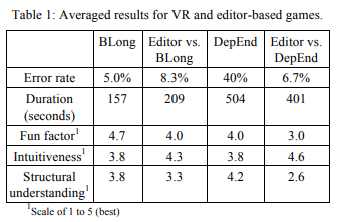
\includegraphics{1}
        \caption{Résultats de l'étude et comparaison}
    \end{figure}

\newpage
\bibliographystyle{plain}
\bibliography{biblio} 
\end{document}